\subsection*{Node2Vec Parameters}

For all experiments, the following parameters hold:
\begin{itemize}
\item For the (\texttt{p=1}, \texttt{q=1})
\item (\texttt{dimensions=16, workers=4})
\item (\texttt{walk\_length=5}, \texttt{num\_walks=300}, \texttt{window=5})
\item (\texttt{min\_count=1}, \texttt{batch\_words=4})
\item (\texttt{EdgeEmbedding=EdgeHadamardEmbedder})
\end{itemize}

\subsection*{XGBoost parameters}
\begin{itemize}
\item \texttt{max\_depth=3}
\item \texttt{colsample\_bytree=0.6}
\item \texttt{eval\_metric='auc'}
\end{itemize}



\subsection*{Supplementary Figures for Human Interactome}

\begin{figure}[h]
\noindent \begin{centering}
\caption{\label{HI1}\emph{HI-II-14} results for \texttt{Node2Vec} with A2
feature}
\par\end{centering}
\noindent \raggedleft{}\includegraphics[width=0.48\columnwidth]{figures/Human/ROC\lyxdot A2}\includegraphics[width=0.48\columnwidth]{figures/Human/CM\lyxdot A2}
\end{figure}

\begin{figure}[h]
\noindent \begin{centering}
\caption{\label{HI2}\emph{HI-II-14} results for \texttt{Node2Vec} with A3
feature}
\par\end{centering}
\noindent \raggedleft{}\includegraphics[width=0.48\columnwidth]{figures/Human/ROC\lyxdot A3}\includegraphics[width=0.48\columnwidth]{figures/Human/CM\lyxdot A3}
\end{figure}

\begin{figure}[h]
\noindent \begin{centering}
\caption{\label{HI3}\emph{HI-II-14} results for \texttt{Node2Vec} with L3
feature}
\par\end{centering}
\noindent \raggedleft{}\includegraphics[width=0.48\columnwidth]{figures/Human/ROC\lyxdot L3}\includegraphics[width=0.48\columnwidth]{figures/Human/CM\lyxdot L3}
\end{figure}

\begin{figure}[h]
\noindent \begin{centering}
\caption{\label{HI1-1}\emph{HI-TESTED} results for \texttt{Node2Vec} with
A2 feature}
\par\end{centering}
\noindent \raggedleft{}\includegraphics[width=0.48\columnwidth]{figures/Human/ROC\lyxdot A2\lyxdot 2}\includegraphics[width=0.48\columnwidth]{figures/Human/CM\lyxdot A2\lyxdot 2}
\end{figure}

\begin{figure}[h]
\noindent \begin{centering}
\caption{\label{HI2-1}\emph{HI-TESTED} results for \texttt{Node2Vec} with
A3 feature}
\par\end{centering}
\noindent \raggedleft{}\includegraphics[width=0.48\columnwidth]{figures/Human/ROC\lyxdot A3\lyxdot 2}\includegraphics[width=0.48\columnwidth]{figures/Human/CM\lyxdot A3\lyxdot 2}
\end{figure}

\begin{figure}[h]
\noindent \begin{centering}
\caption{\label{HI3-1}\emph{HI-TESTED} results for \texttt{Node2Vec} with
L3 feature}
\par\end{centering}
\noindent \raggedleft{}\includegraphics[width=0.48\columnwidth]{figures/Human/ROC\lyxdot L3\lyxdot 2}\includegraphics[width=0.48\columnwidth]{figures/Human/CM\lyxdot L3\lyxdot 2}
\end{figure}

\begin{figure}[h]
\noindent \begin{centering}
\caption{\label{F8-importance-H2}Importance gain plots for \emph{HI-TESTED}}
\par\end{centering}
\begin{centering}
\includegraphics[width=0.7\columnwidth]{figures/Human/Imp\lyxdot A2\lyxdot 2}
\par\end{centering}
\begin{centering}
\includegraphics[width=0.7\columnwidth]{figures/Human/Imp\lyxdot A3\lyxdot 2}
\par\end{centering}
\centering{}\includegraphics[width=0.7\columnwidth]{figures/Human/Imp\lyxdot L3\lyxdot 2}
\end{figure}


\subsection*{Supplementary Figures for Rice Interactome}

\begin{figure}[h]
\noindent \begin{centering}
\caption{\label{F2}Results for \texttt{Node2Vec} with A2 feature}
\par\end{centering}
\noindent \raggedleft{}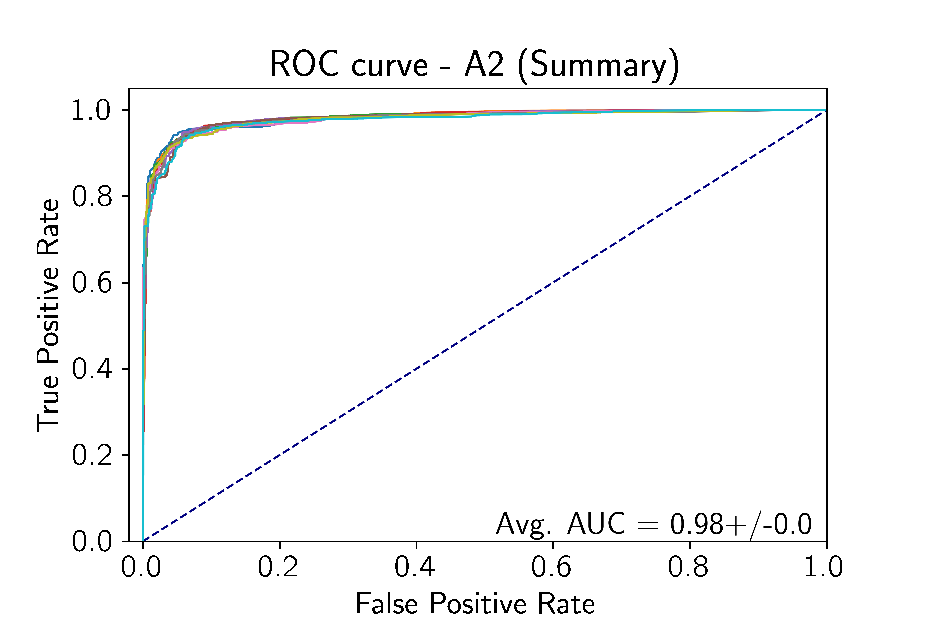
\includegraphics[width=0.48\columnwidth]{figures/ML_Metric/ROCA2_SUMMARY}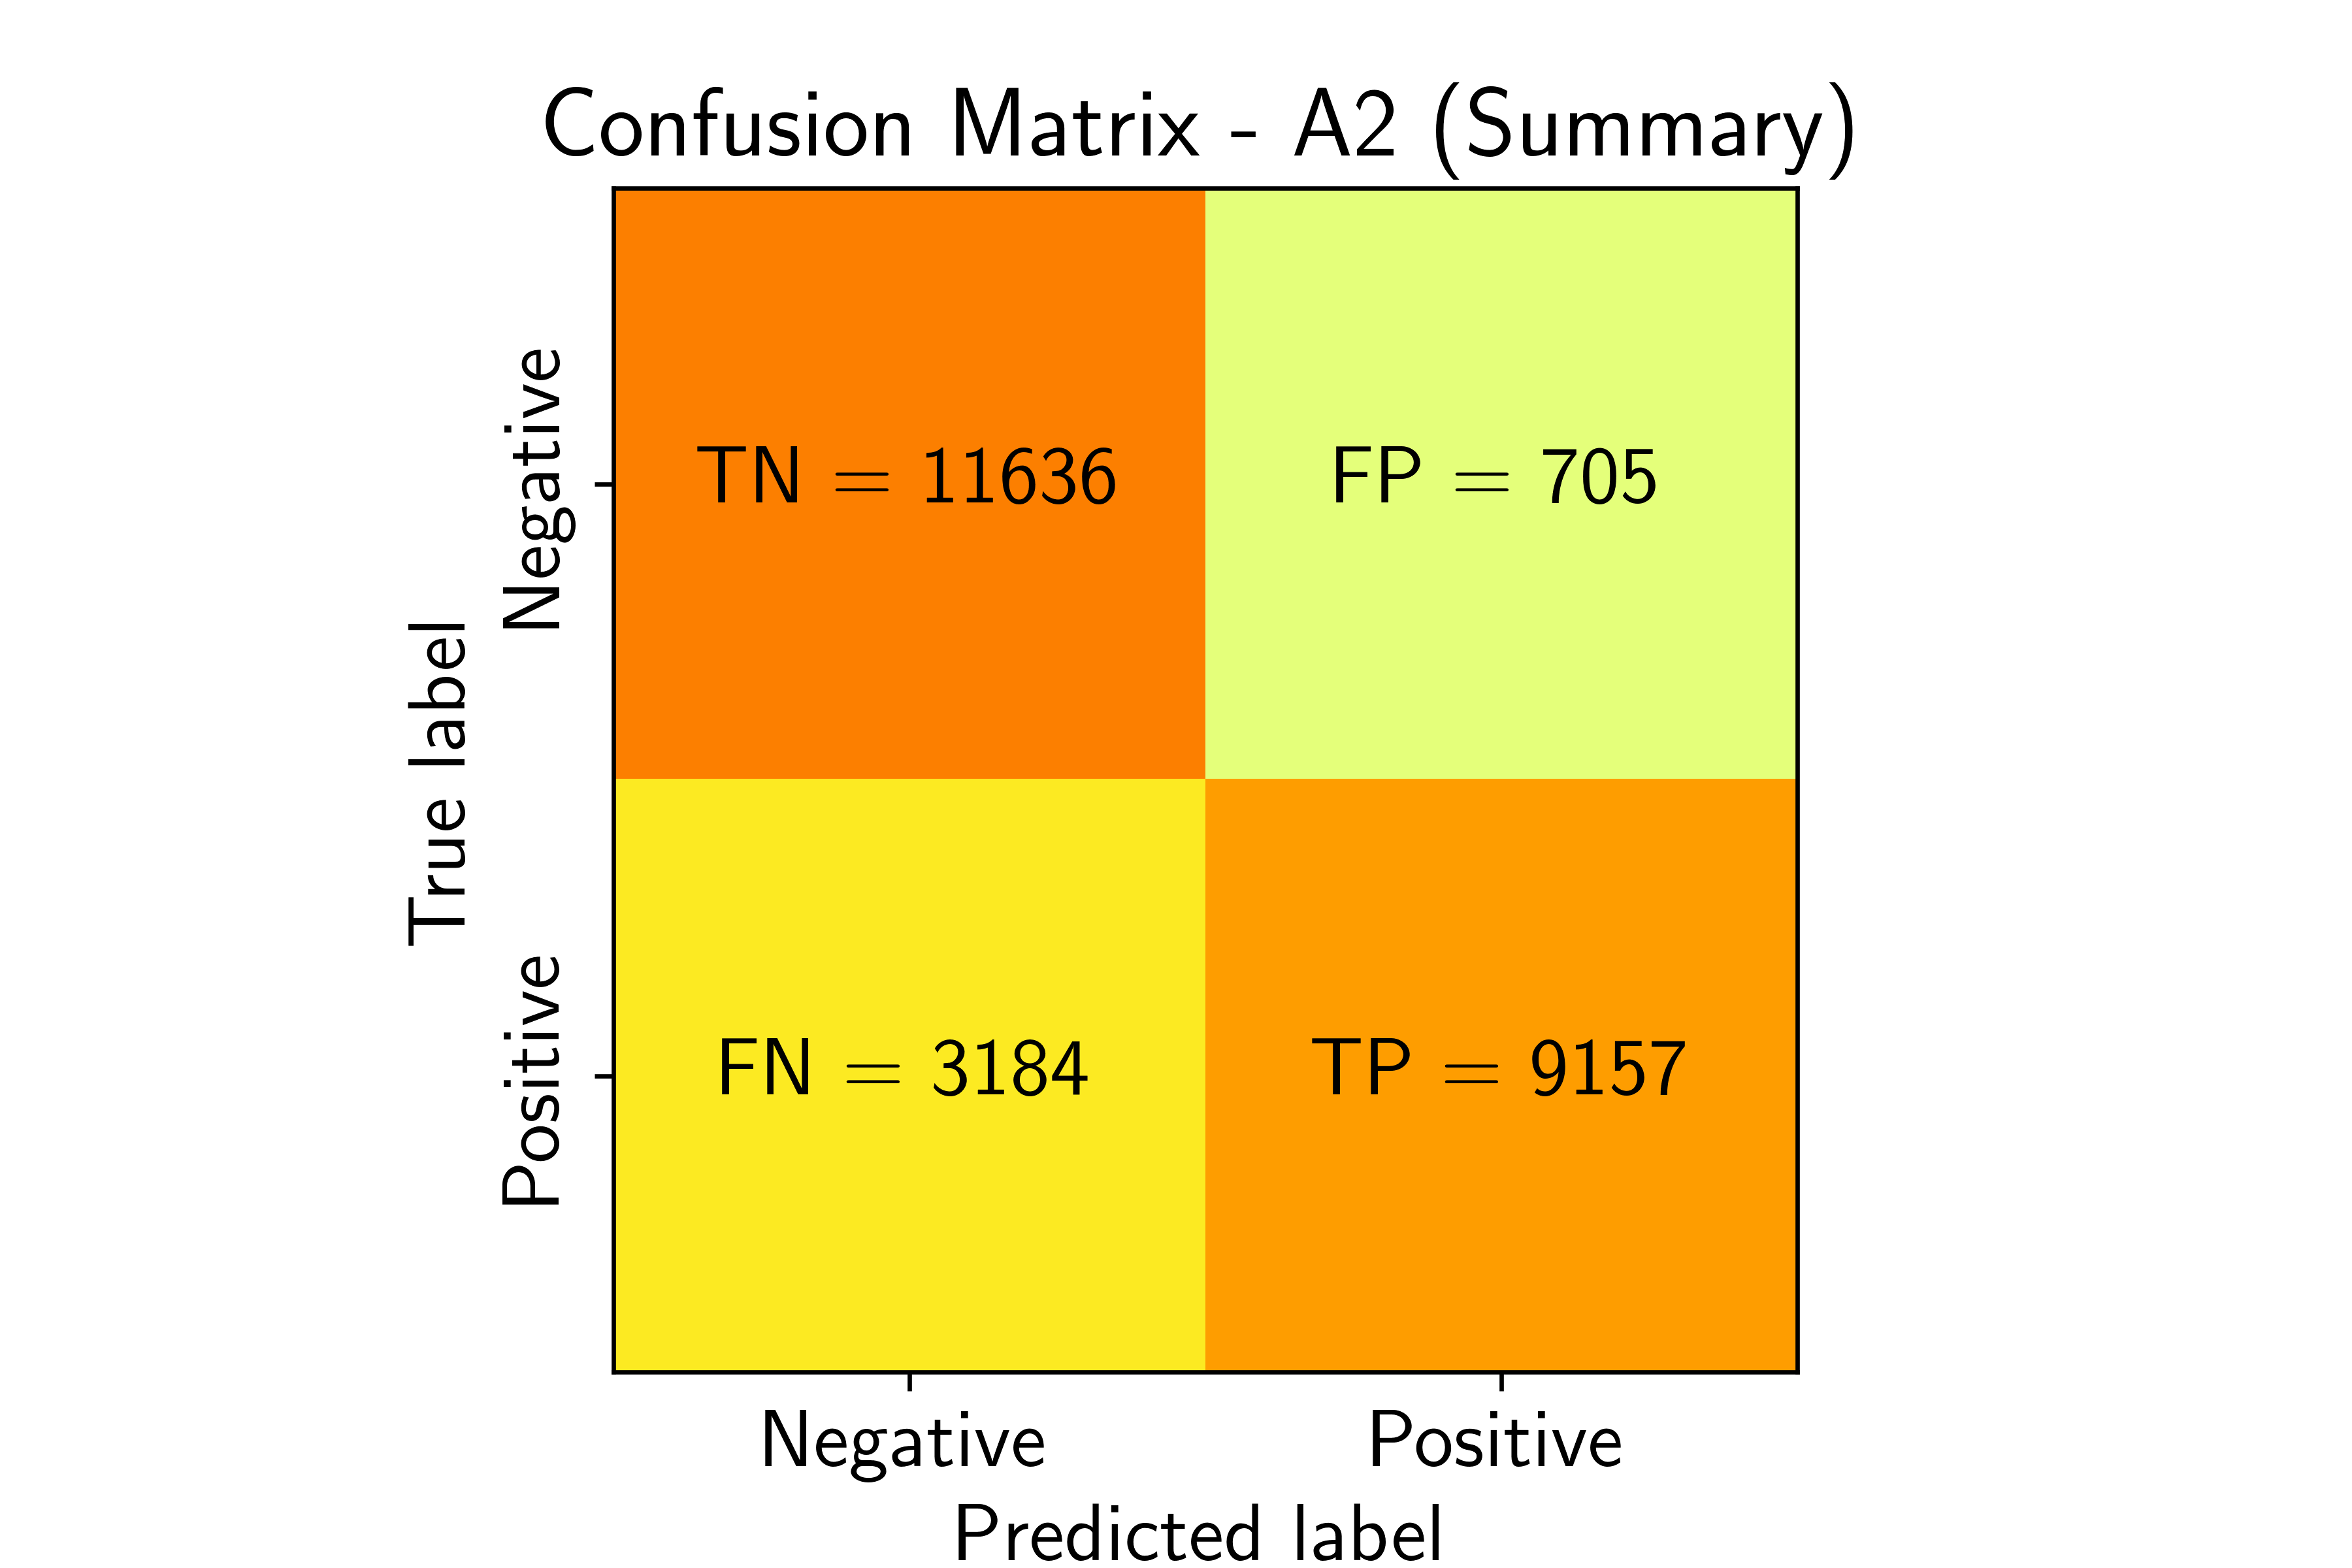
\includegraphics[width=0.48\columnwidth]{figures/ML_Metric/CMA2_SUMMARY}
\end{figure}

\begin{figure}[h]
\noindent \begin{centering}
\caption{\label{F3}Results for \texttt{Node2Vec} with A3 feature}
\par\end{centering}
\noindent \raggedleft{}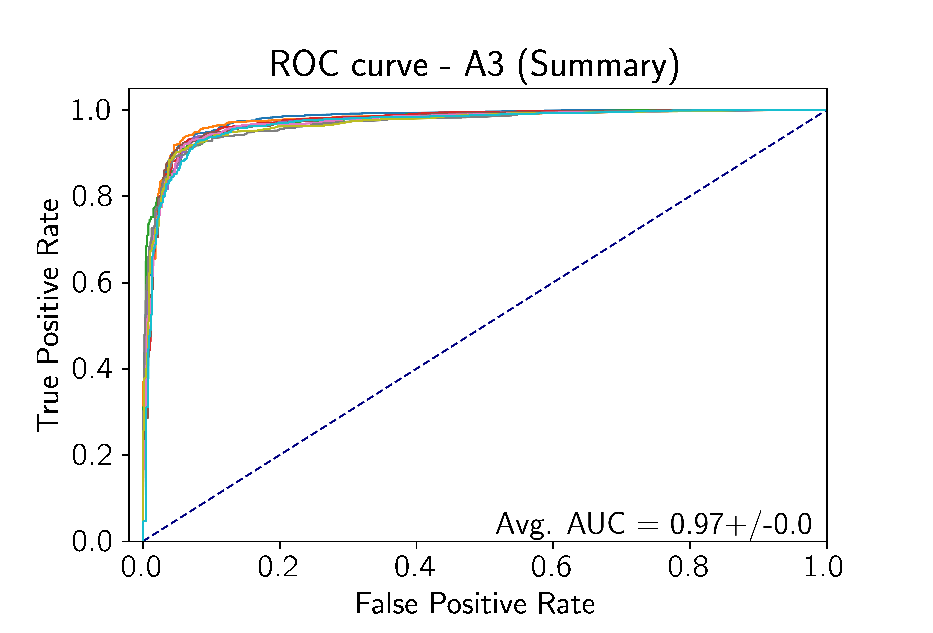
\includegraphics[width=0.48\columnwidth]{figures/ML_Metric/ROCA3_SUMMARY}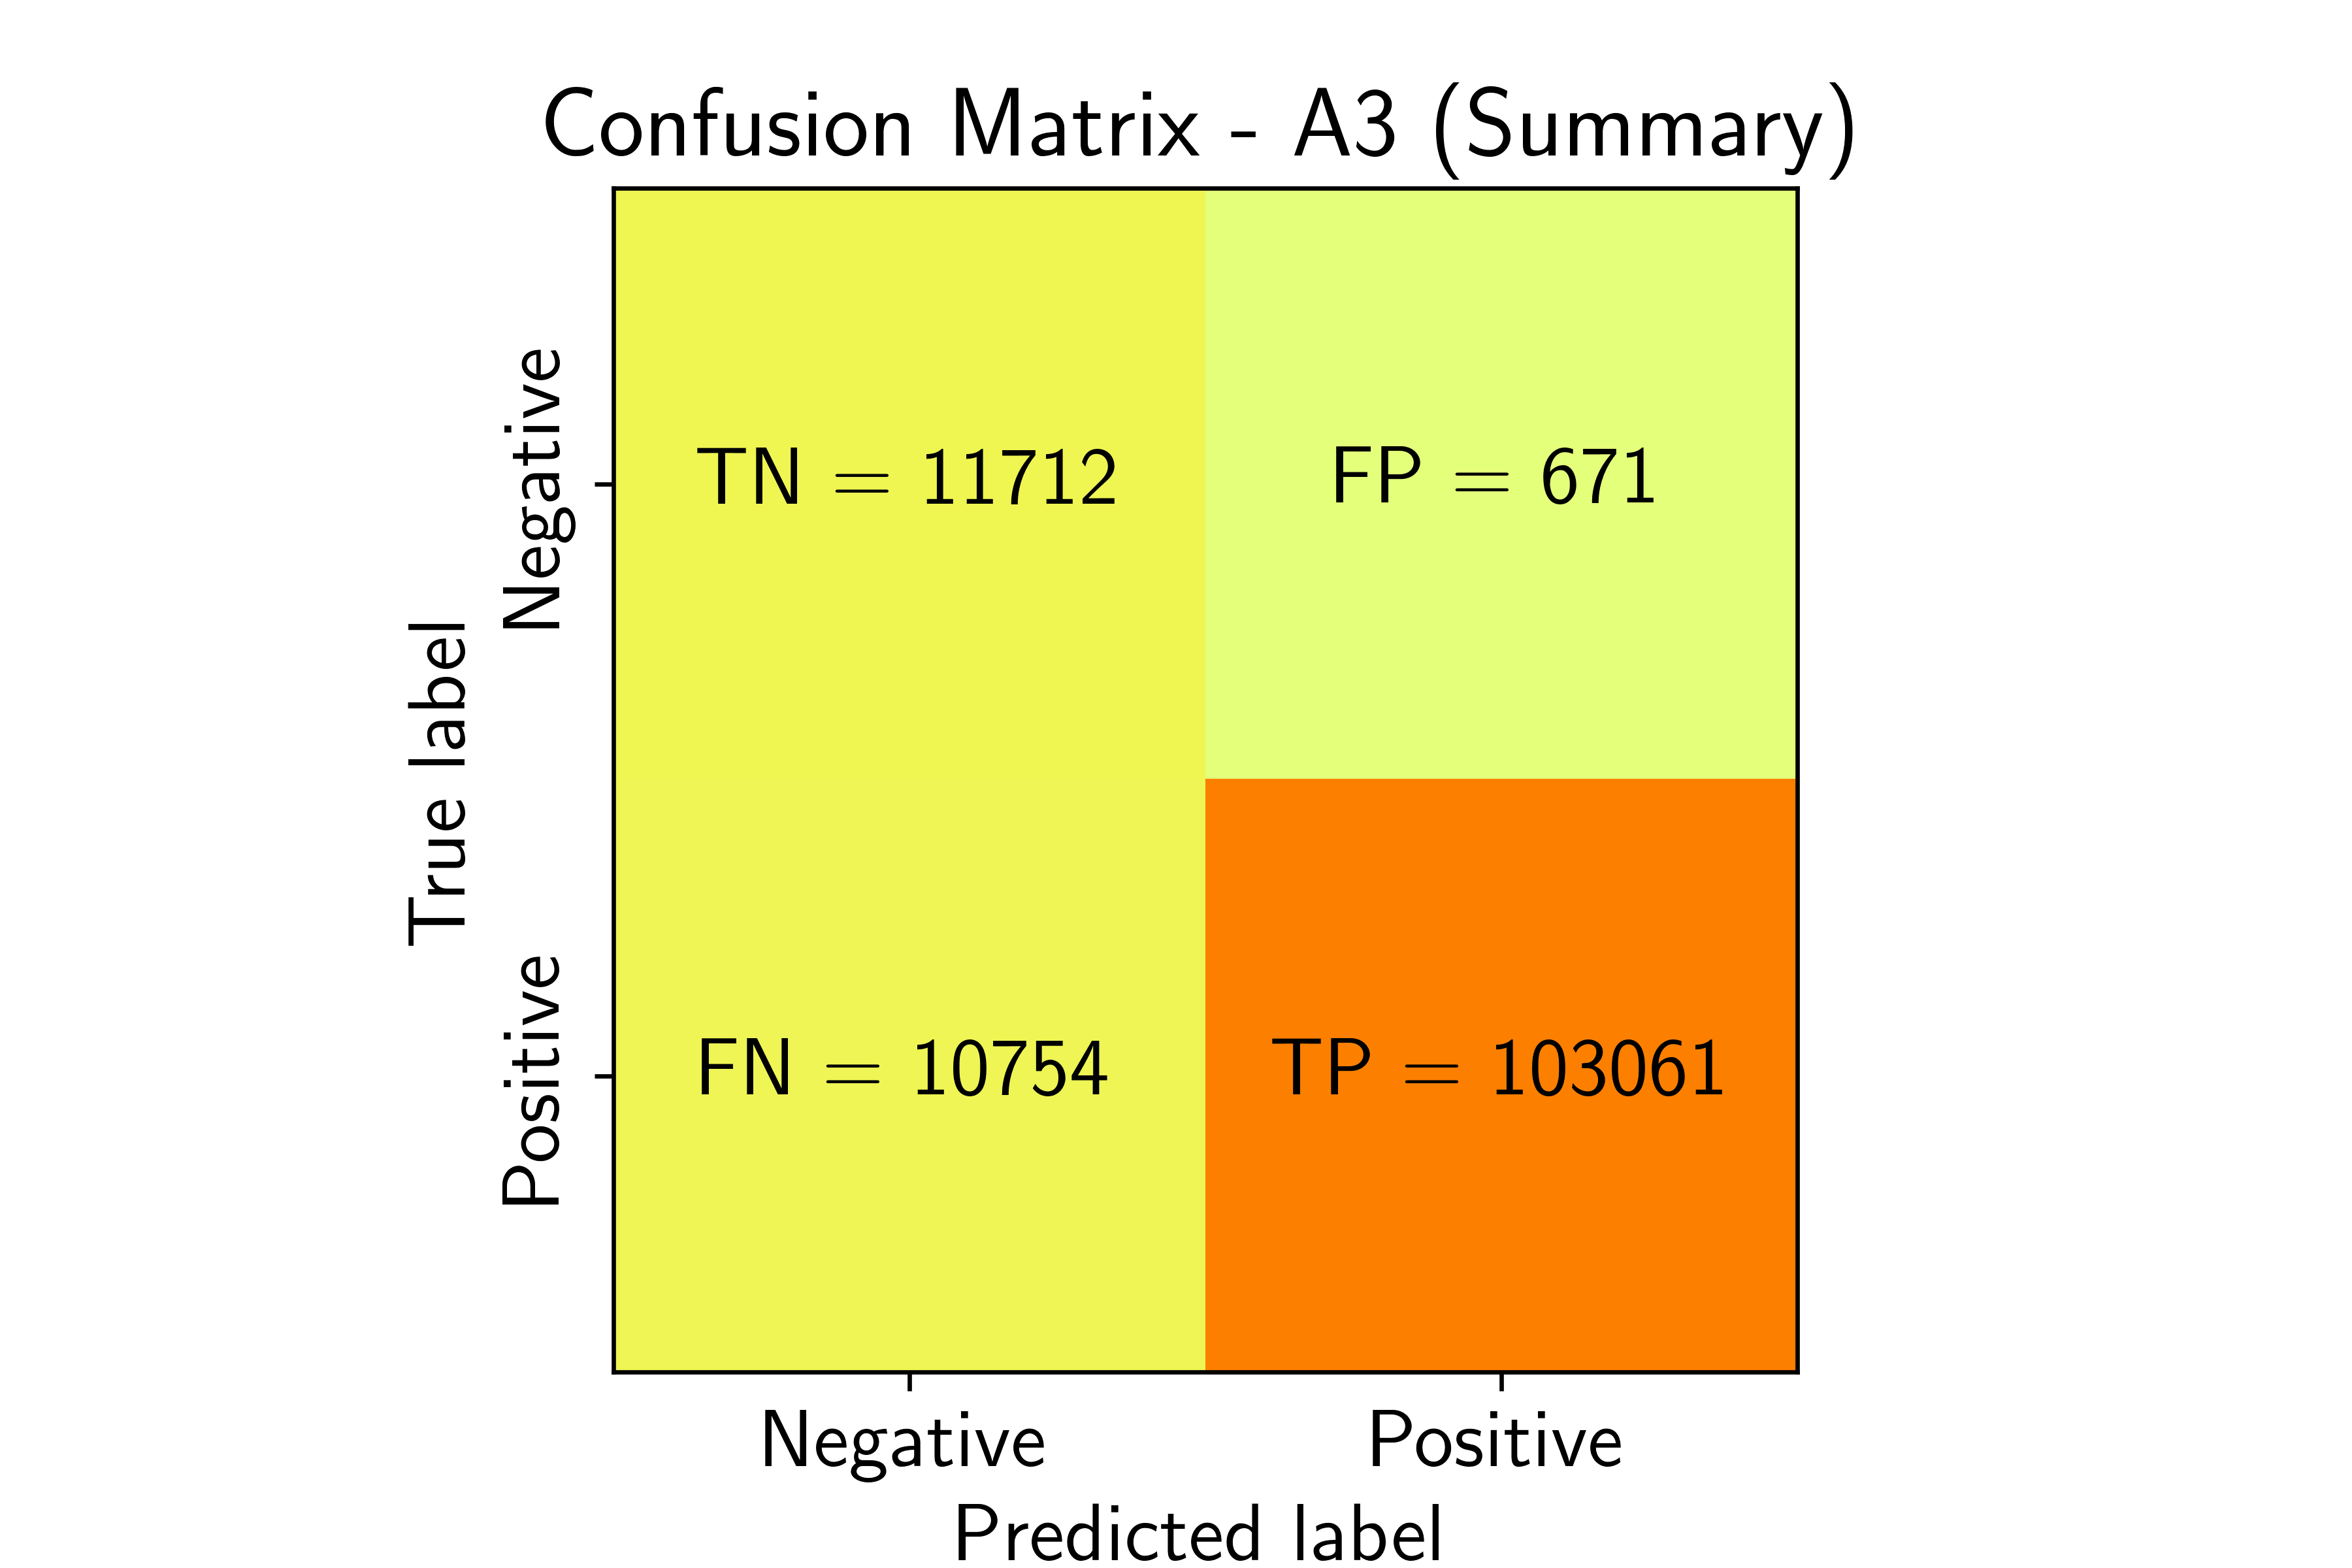
\includegraphics[width=0.48\columnwidth]{figures/ML_Metric/CMA3_SUMMARY}
\end{figure}

\begin{figure}[h]
\noindent \begin{centering}
\caption{\label{F5}Results for A2 feature only}
\par\end{centering}
\noindent \raggedleft{}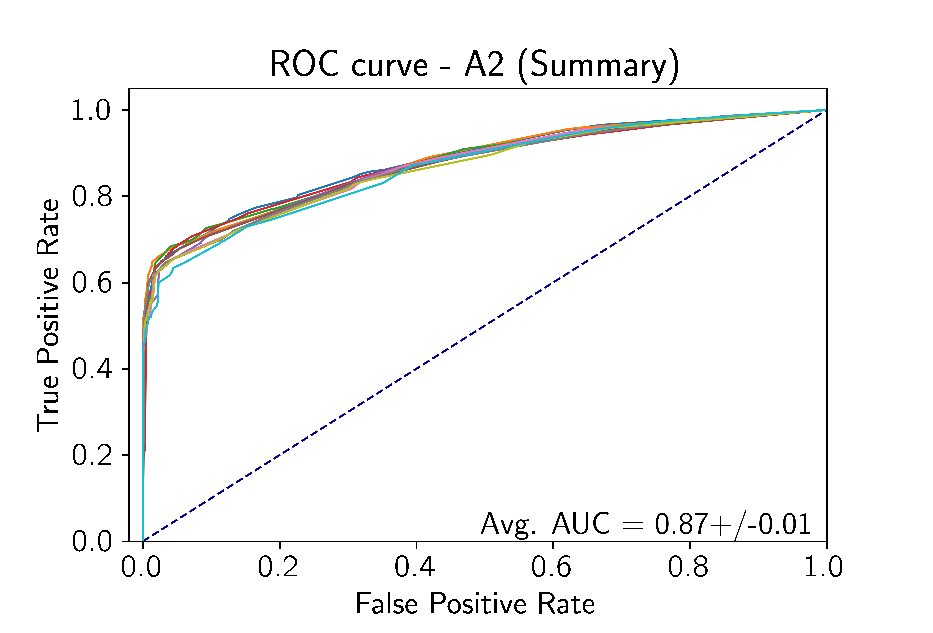
\includegraphics[width=0.48\columnwidth]{figures/Only_Metric/ROConlyA2_SUMMARY}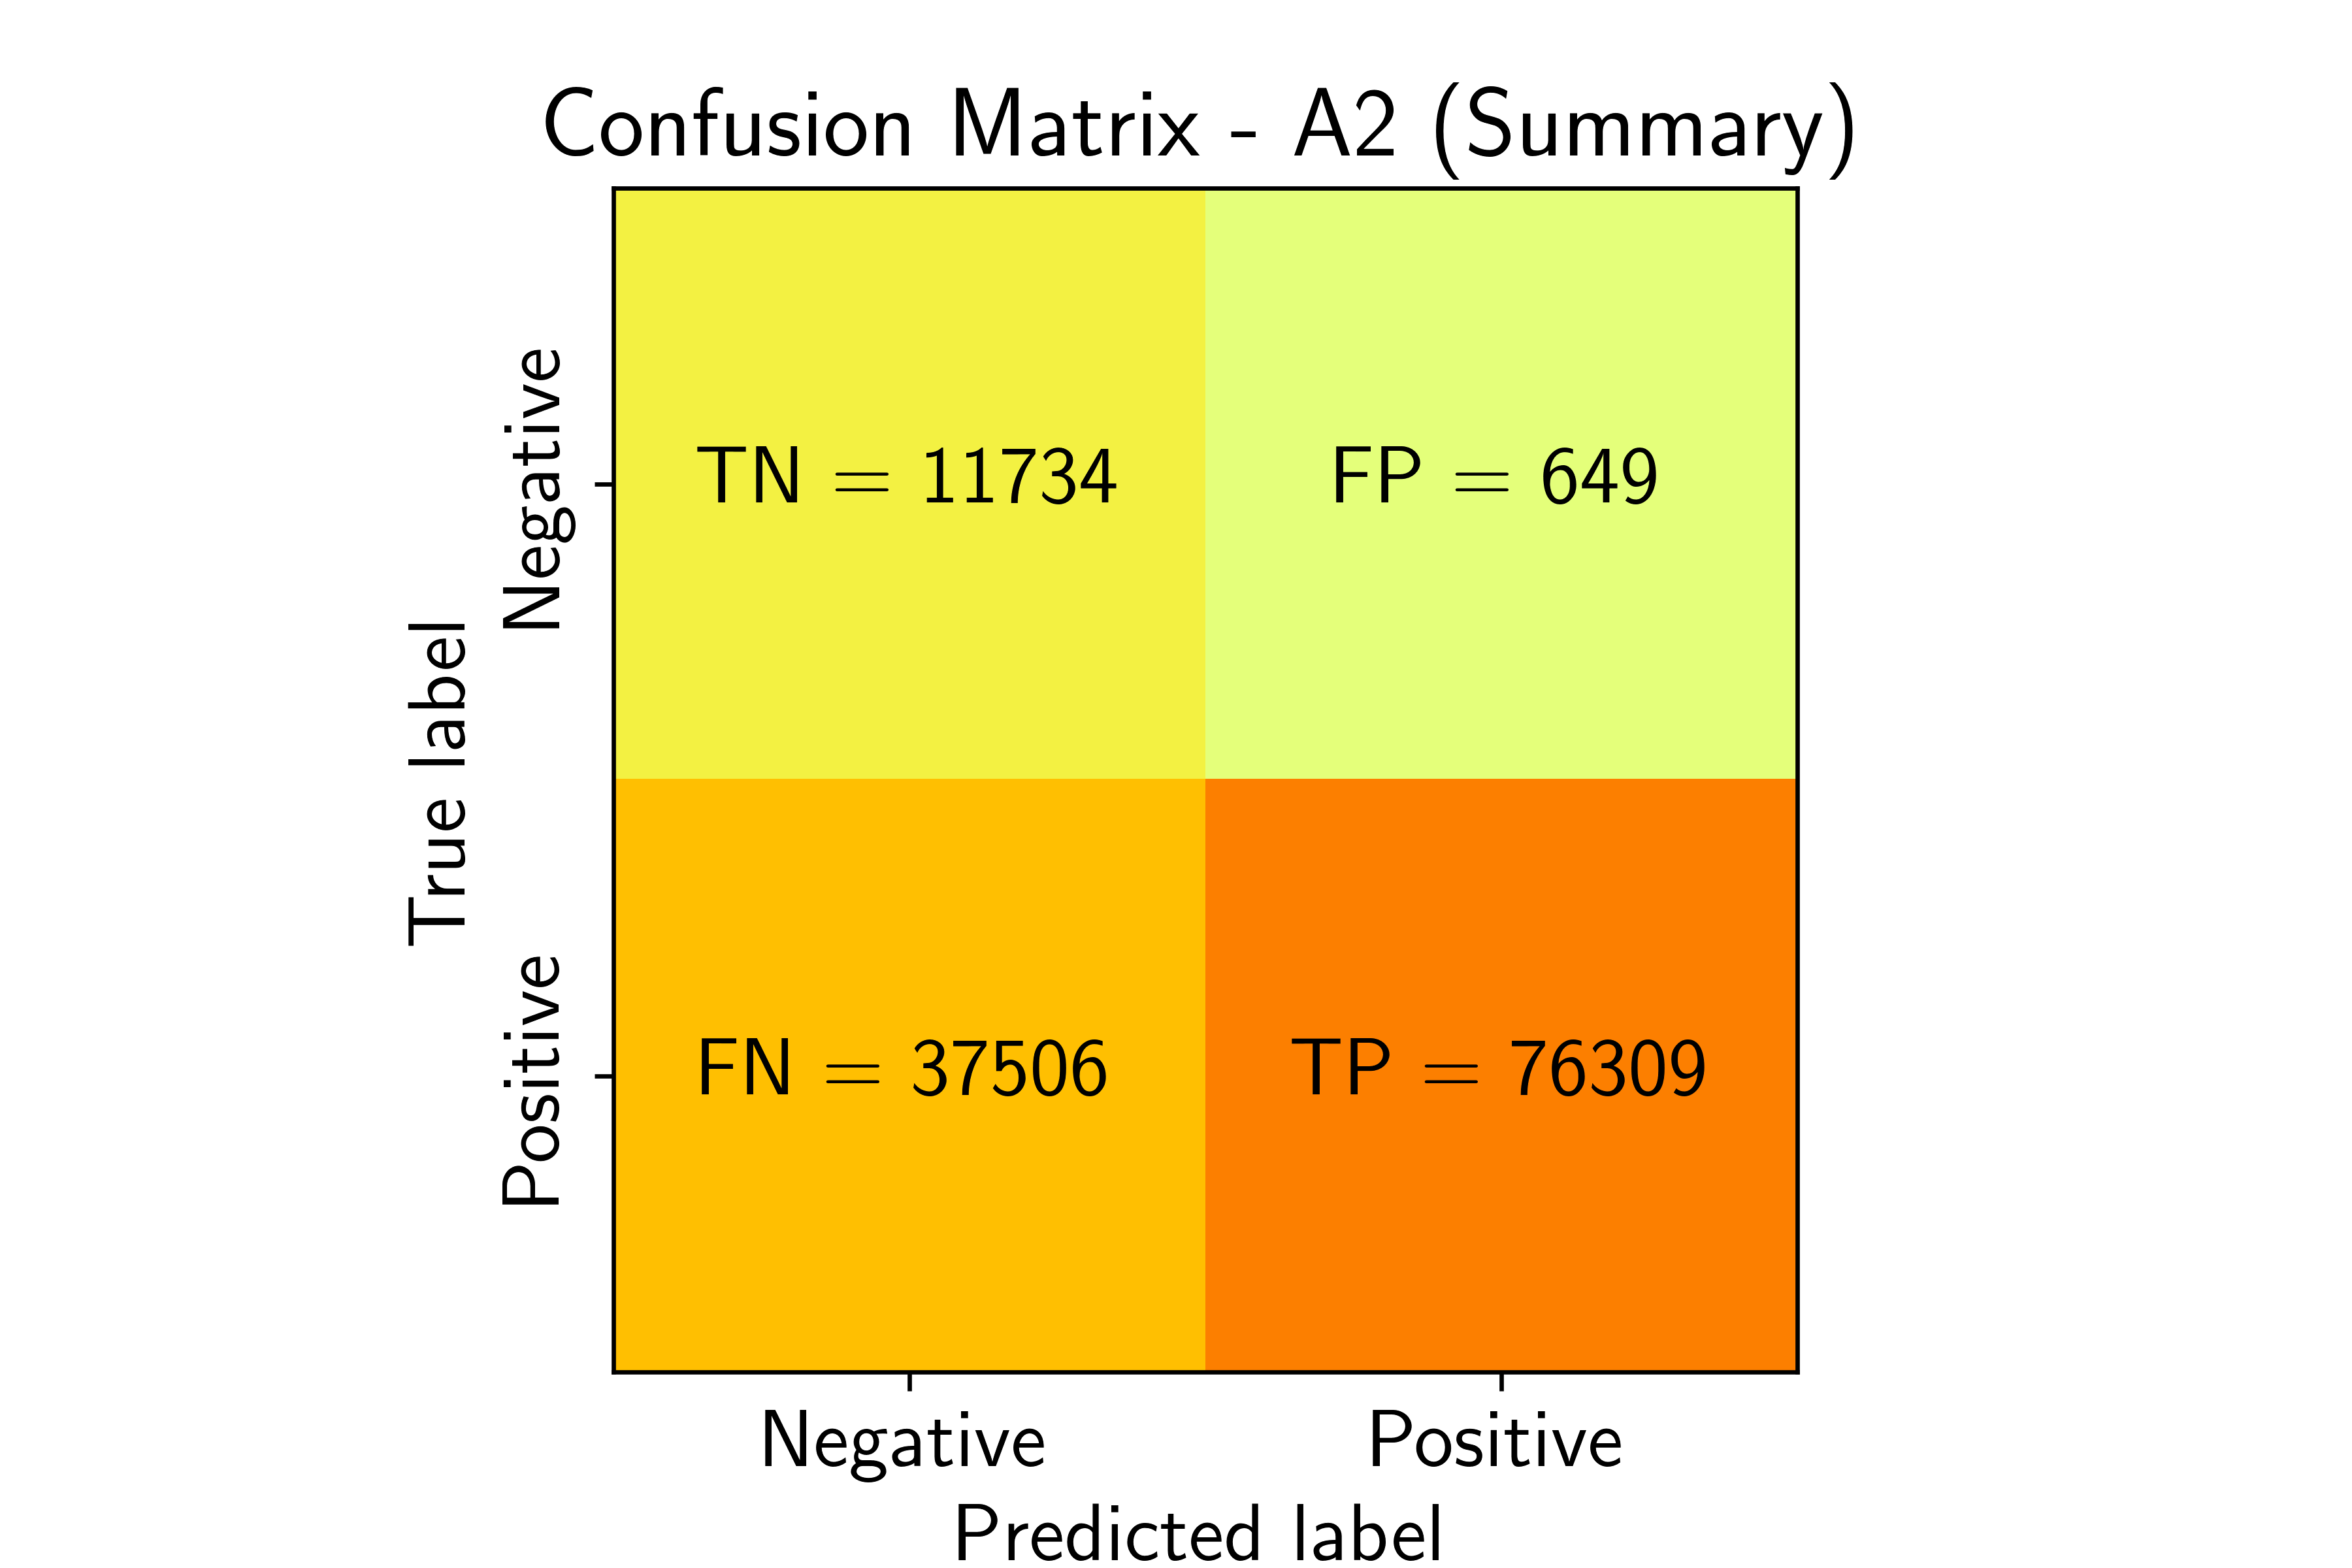
\includegraphics[width=0.48\columnwidth]{figures/Only_Metric/CMonlyA2_SUMMARY}
\end{figure}

\begin{figure}[h]
\noindent \begin{centering}
\caption{\label{F6}Results for A3 feature alone}
\par\end{centering}
\noindent \raggedleft{}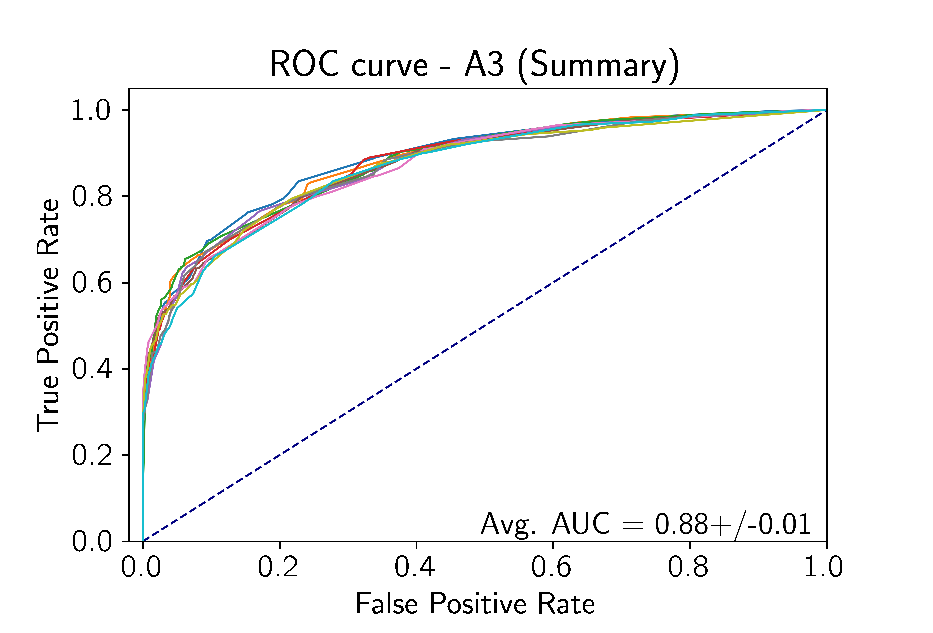
\includegraphics[width=0.48\columnwidth]{figures/Only_Metric/ROConlyA3_SUMMARY}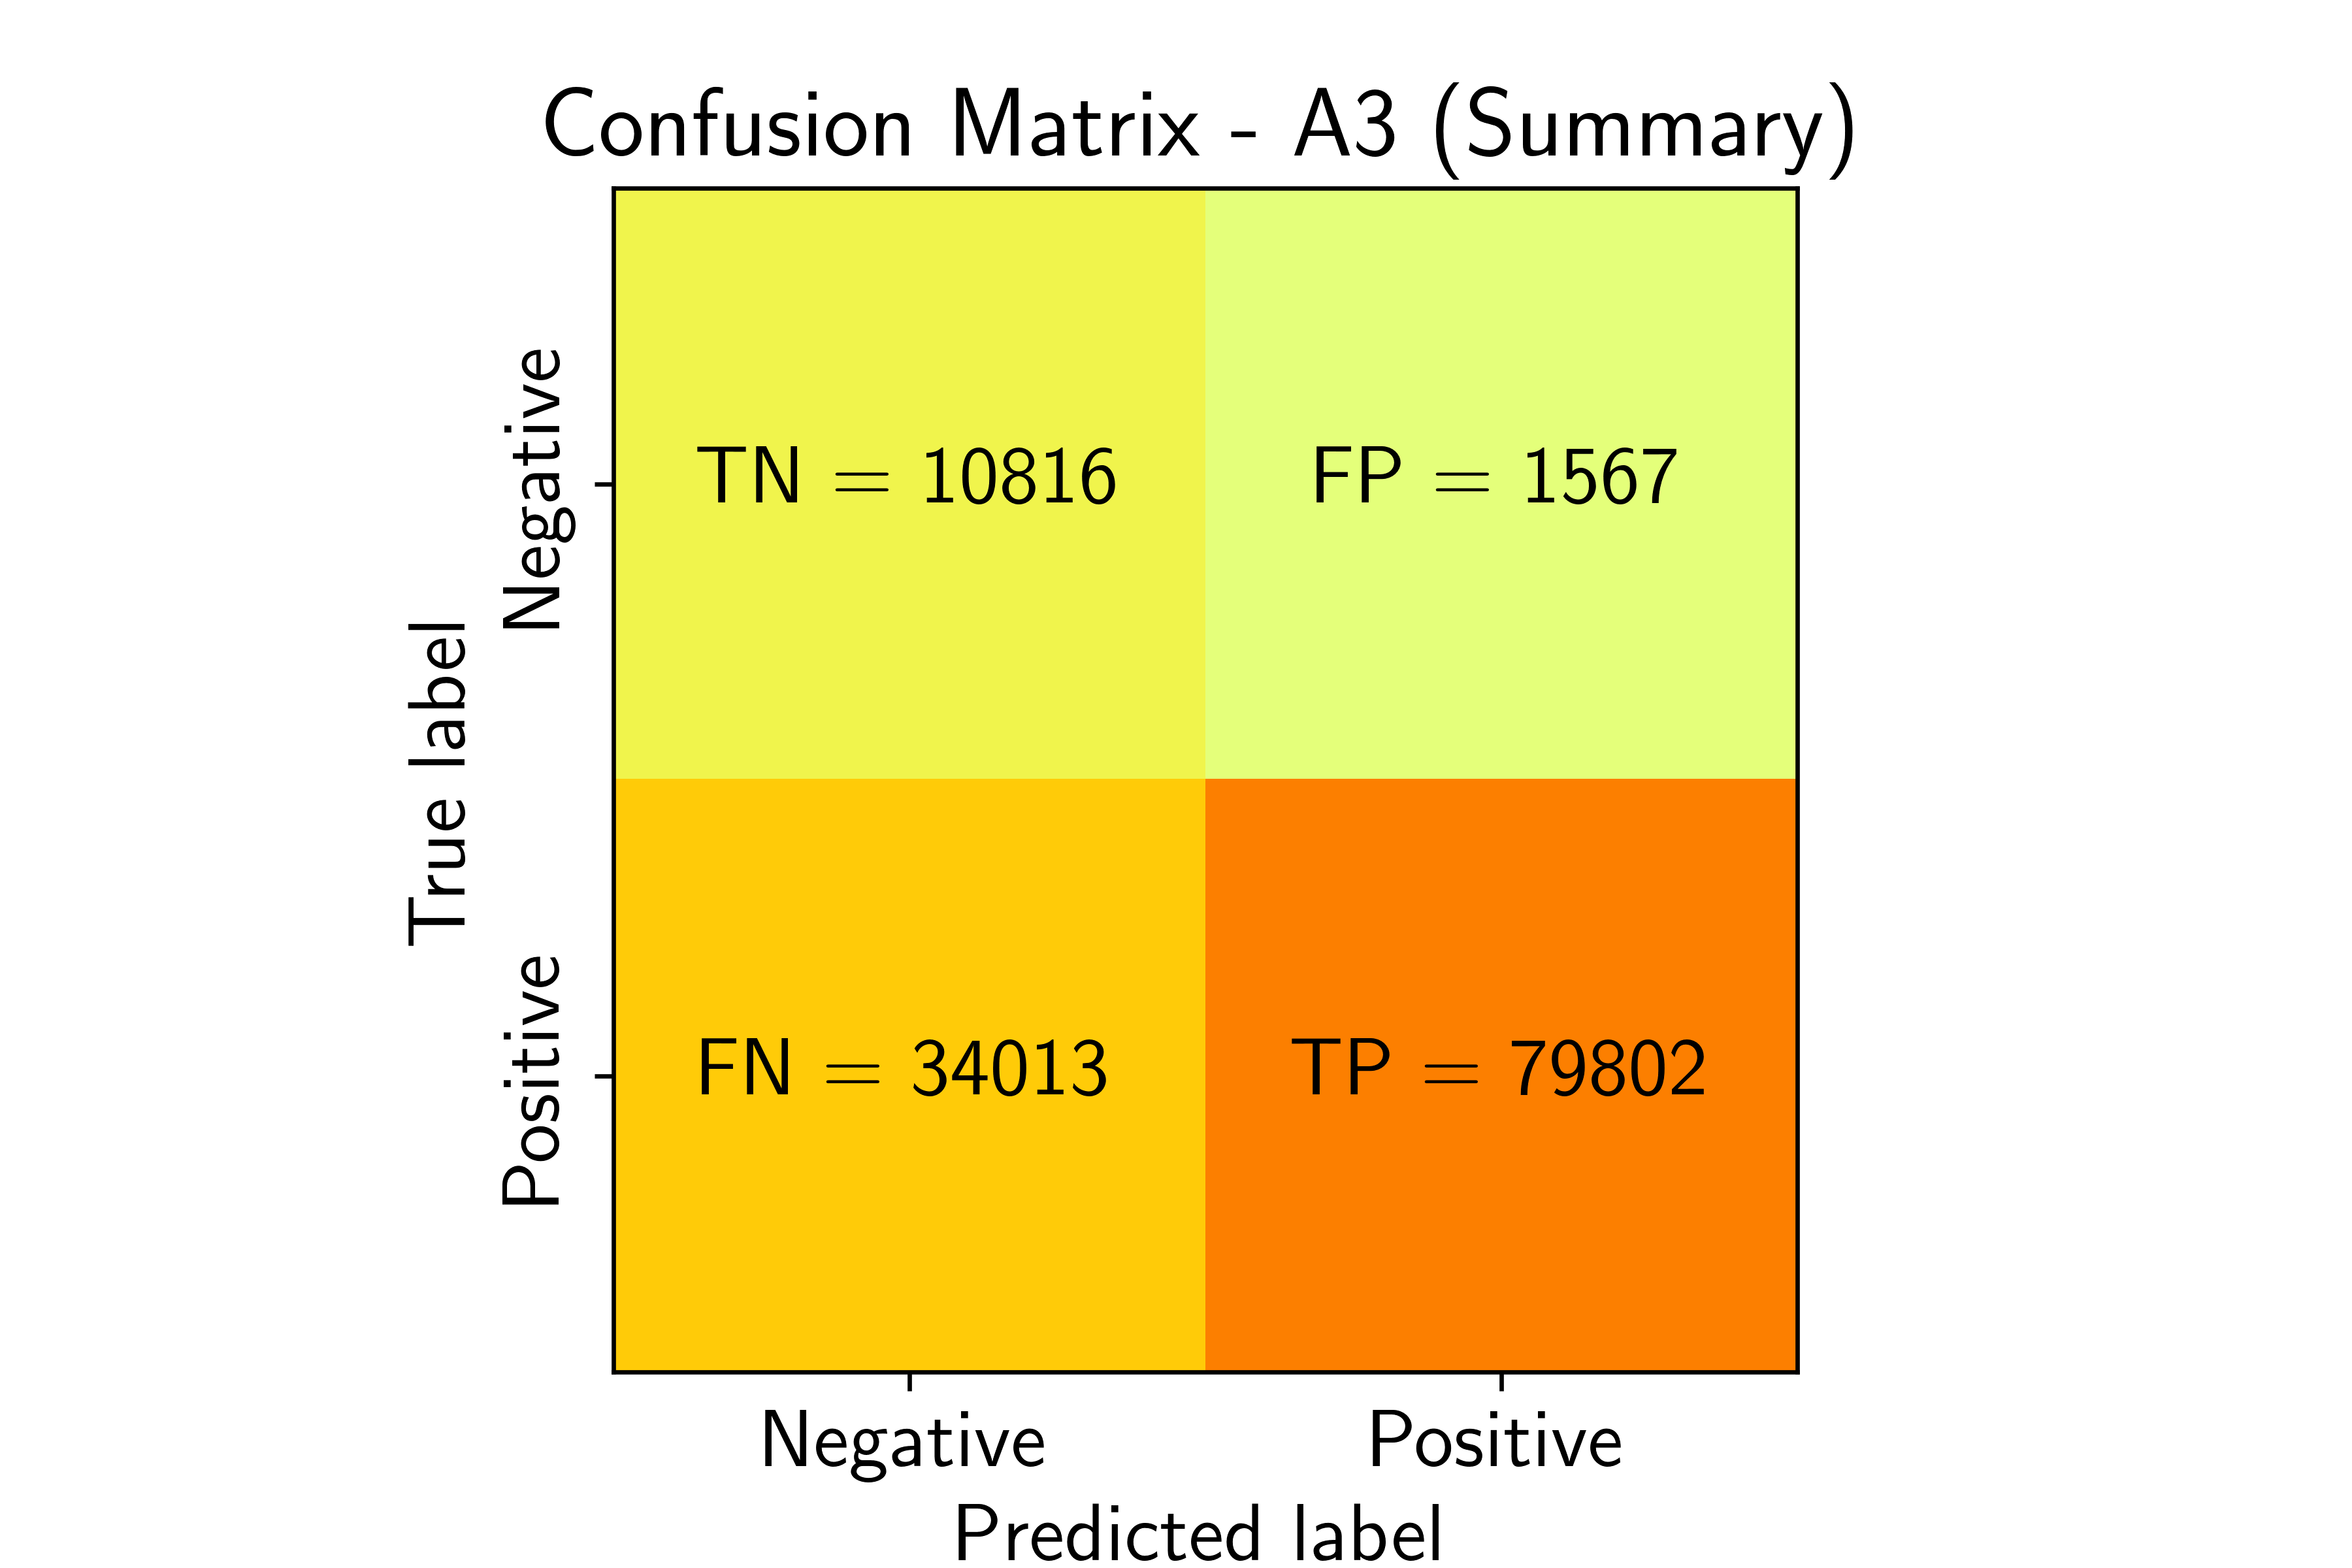
\includegraphics[width=0.48\columnwidth]{figures/Only_Metric/CMonlyA3_SUMMARY}
\end{figure}
